\chapter{Batteries}
To operate the car is required two main source of power coming from two distinct sets of batteries. The main battery is an high voltage \gls{DC} pack. To activate it is necessary a 24V source. For that is required a secondary power source, where it is extracted the low voltage.
They contain a \gls{BMS} managed by a micro controller with whom the user interacts to activate the high voltage section and get information about the status of battery. The communication is performed via CAN interface.

Currently is used two independent set of batteries to provide low voltage. A pack with 24V and another with 12V. However is currently in study and design a single pack with 48V  of nominal voltage with integrated \gls{BMS} to unify the low voltage source and intermediate \gls{DC}-\gls{DC} switching converters will be used to provide 24V and 12V rails.

\section{Main battery packs}
The power train battery consists in two interconnected battery packs each other with 72 individual cells. Both pack are connected in series deploying the total voltage for the Siemens power inverter. The battery pack specifications are present in table \ref{tab:battery_pack_specs}. The main battery connections are shown in figure \ref{fig:battery_connections} In orange is seen the high voltage connectors and the black ones are the low voltage and also control system connectors. 

\begin{figure}[!h]
	\centering
	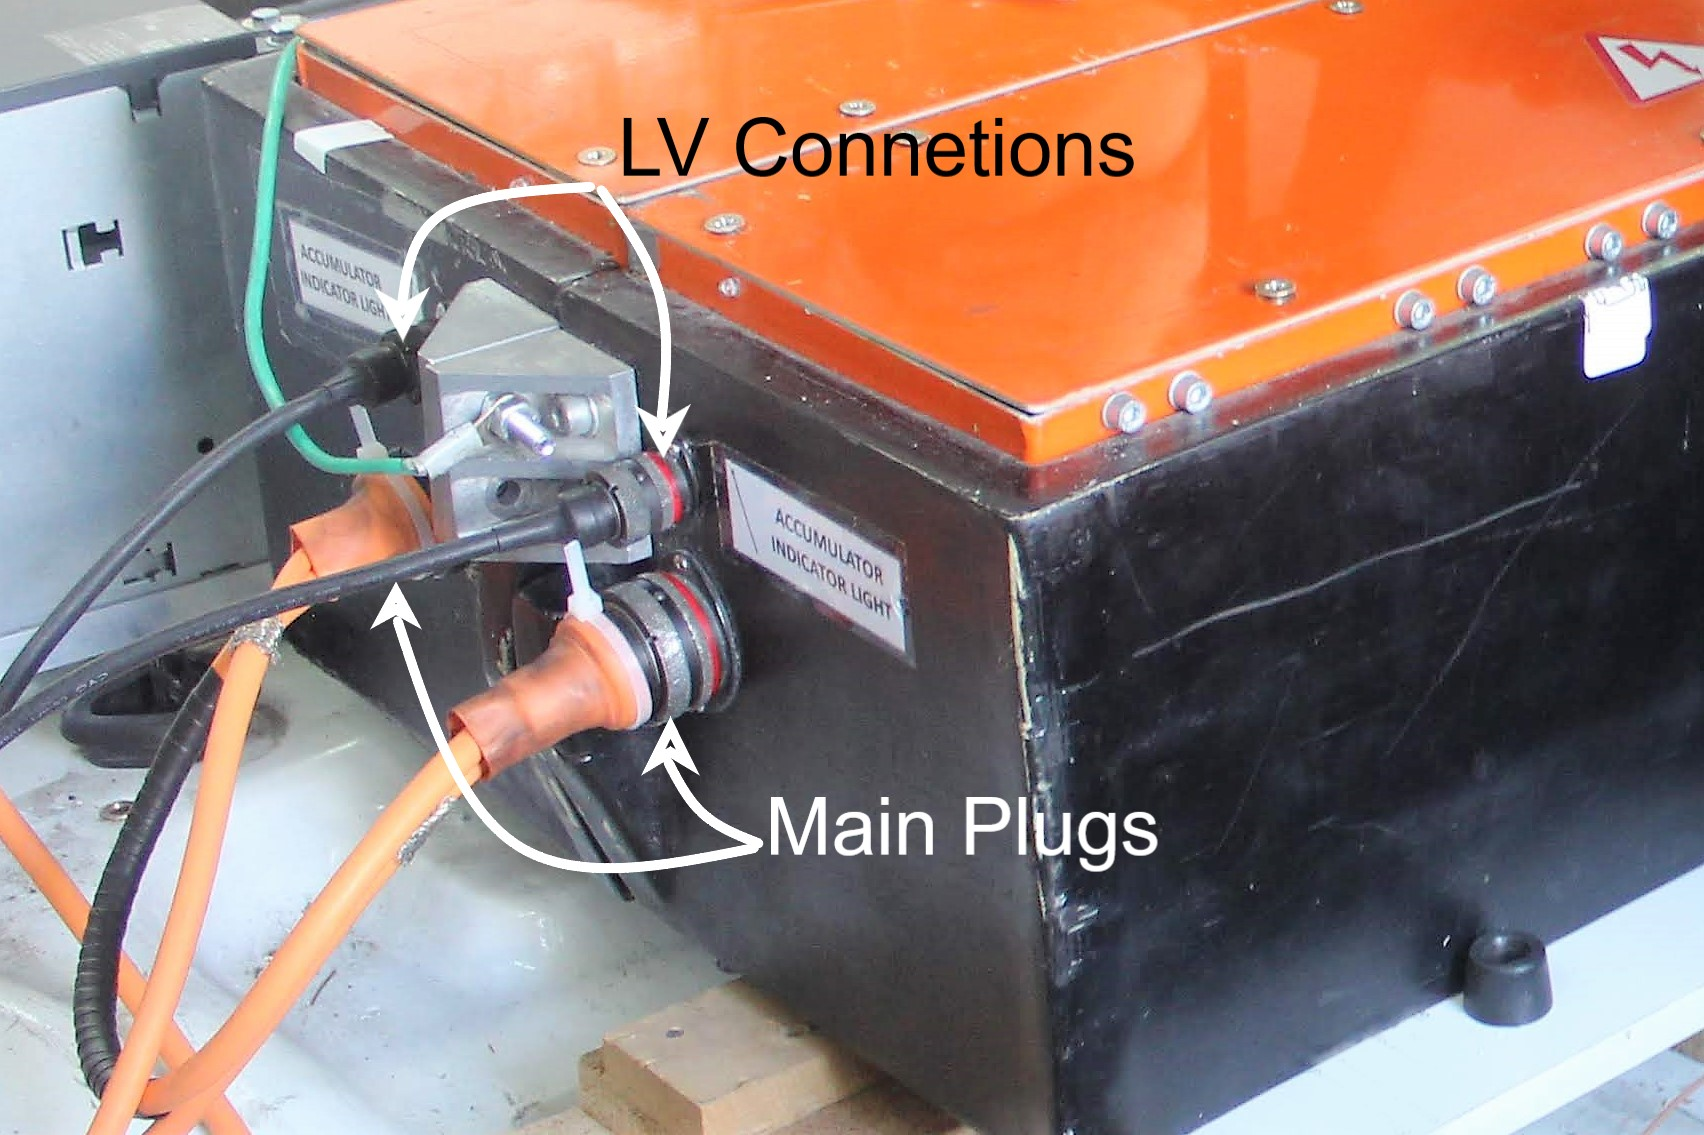
\includegraphics[width=0.7\linewidth]{figures/main_battery_connections}
	\caption{Main batterry pack and connectors}
	\label{fig:battery_connections}
\end{figure}

\begin{table}
	\centering
	\begin{tabular}{lc}
		\toprule
		\textbf{Parameter} & \textbf{Value}\\
		\midrule
		Maximum tractive system voltage & 600 V \\
		Nominal tractive system voltage & 532,8 V \\
		Control system voltage & 24 V \\
		Accumulator configuration & 144s1p \\
		Total accumulator capacity & 10 Ah\\
		\bottomrule
	\end{tabular}
	\caption[Battery pack specifications]{Battery pack specifications (source \cite{fst06})}
	\label{tab:battery_pack_specs}
\end{table}

\subsection{Connections}
The low voltage connectors contain 22 numbered pins listed in table \ref{tab:lv_connections} with respective description of them plus the expected connection. The expected connection is not the original intended connection signal since they were designed for use within \gls{FST} championships and have to oblige several protections like automatic cut power in case of water leakage detection inside specific compartments for instance. Majority of those rules, do not apply for our case. As so, all \gls{AIR} feeds are connected to 24V. Basically \gls{AIR} feeds act similar to a series of safety interrupters that must be active to provide high voltage but in this case is bypassed. Description of pins were provided by \gls{FST} members.

\begin{mdframed}[backgroundcolor=red!20, roundcorner=10pt, innertopmargin=5pt, innerbottommargin=5pt, skipabove=5pt]
	\Warning \, \textbf{The CAN connections are not internal terminated with the 120 $\Omega$ resistor.}
\end{mdframed}

\begin{table}
	\centering
	\begin{tabular}{cclcc}
		\toprule
		\textbf{Group} & \textbf{Pin Number} & \textbf{Description} & \textbf{Cable color} & \textbf{Value}\\
		\midrule
		% group supply
		\multirow{2}{*}{Supply}& 1 & GND     & yellow & GND	\\
		 & 2 & VCC\_A1 & white  & 24V \\
		 \midrule
		 & 3 & \multicolumn{3}{c}{Not used} \\
		 \midrule
		 % group AIR
		 \multirow{2}{*}{AIR} & 4 & AIR     & white  & 24V \\	
		 & 5 & AIR     & white  & 24V \\
		 % group AIR_supply
		 \midrule
		 \multirow{2}{*}{AIR Supply}& 6 & GND	    & yellow & GND \\
		 & 7 & VCC\_AIR  & white  & 24V \\
		 % group Fans
		 \midrule
		 Fans & 8 & GND	    & yellow & GND \\
		 (not used in this version) & 9 & VCC\_AIR  & white  & 24V \\
		 \midrule
		 \vspace{1pt}\\
		 \multicolumn{5}{c}{Pins 10 to 19 are not used}\\
		 \vspace{1pt}\\
		 \midrule
		 \multirow{2}{*}{CAN}& 20 & CAN\_L & Black & CAN Low \\
		 & 21 & CAN\_H  & Black  & CAN High \\
		 \midrule
		  & 22 & \multicolumn{3}{c}{Not used} \\
		\bottomrule
	\end{tabular}
	\caption{Main battery low voltage connections description}
	\label{tab:lv_connections}
\end{table}

\subsection{Power requirements}
When active, the main battery pack draws near 3A of current majority of them used in the activation of high voltage relays. The auxiliary pack must be able to support such need.

\subsection{List of CAN messages}
\blindtext

\subsection{Enabling power}
\blindtext

\section{Auxiliary battery pack}
\blindtext

